% vim: set ts=2 sw=2 noet spell:

\chapter{Conclusions} \label{chp:conclusions}

\section{Results}

The goal to build a functional demonstrator had been achieved, unfortunately not all of the originally planned features were implemented. A stable wireless link using QPSK modulation that computes the BER was developed.

Some different typ of multiple fading model were tested and illustrated.
Two different Models for the simulation options are built. One discrete time model whish is  basically a FIR filter in the channel, the other with a statistical model which is based on a GR block.

One other file to implement the hardware with. Unfortunately it was not possible to measure those in a meaningful way. For that a least square approximation could be used as described in the further steps. An other difficulty is to reproduce the same effect in a simulation compare with the hardware, because of al the side effect of the environment, which cant be predicted in a simulation.

% TODO Mention QAM16 

\section{Future Work}

\subsection{Improve BER measurements and simulations}

A missing feature in this work is an automated collection of the BER data, which would allow to more easily to observe and measure the influence of each parameters in the fading channel model.

\subsection{Improvements of GUI frontend}

The current GUI prototype built with DearPyGUI has some issues, the most critical begin a single-threaded application. The interprocess communication (with GR's flow graphs) should be on a separate thread from the graphics. The problem is not noticeable as long as the flow graphs in the background keep sending data, but as soon as the UDP/IP data stream stops the timeout of the socket interface causes the interface to run at less that 20 frames per second.

In addition to fixing the aforementioned issue, a very important feature that is currently missing is the ability to change the fading parameters in real time from within the GUI. Dear PyGUI offers many graphical elements that could be used to control the parameters, however a new GR block would need to be created to propagate the updated values into the flow graph.

\subsection{Channel parameters estimation with Pilot Symbols}

An interesting continuation of this work could be to regularly interpolate some so called pilot symbols in the modulated data stream. Briefly, the pilot symbol assisted modulation (PSAM) technique consists of periodically inserting informationless (known) symbols in the data stream, which are then used to estimate the fading parameters of the communication channel. More details are presented in \cite{Xiaoyi1999} (and its references) from which the illustrations in \figref{fig:psam} were taken.

\begin{figure}
	\centering
	\includegraphics[width = \linewidth]{figures/xiaoyi-psam-figures}
	\caption{
		Illustration of the pilot symbols assisted modulation (PSAM) frame format (left), and PSAM fading interpolation method (right). The PSAM technique allows to compute the fading (denoted in the figure with \(\tilde{z}_n\)) by interpolating measurements of informationless symbols (pilot symbols) over multiple frames. Both figures were taken from \cite{Xiaoyi1999}, which presents an analytical method to compute the BER from the PSAM and multilevel quadrature amplitude modulation (M-QAM) parameters.
		\label{fig:psam}
	}
\end{figure}

\section{Closing words}

\section{Acknowledgments}


We would like to thank everyone who took the time to help us. Specially Michel Nyffenegger, Nicola Ramagnano for their explanations, with the GNU Radio tool,
Marcel Kluser, who has provided the equipment, Prof. Dr. Heinz Mathis for the opportunity and to our friends whose supported us in different ways.



